\vspace{10pt}

{\centering\subsection*{孙媛媛:变形记}}

\addcontentsline{toc}{subsection}{孙媛媛:变形记}

\renewcommand{\leftmark}{孙媛媛:变形记}

\begin{figure}[htbp]

\centering

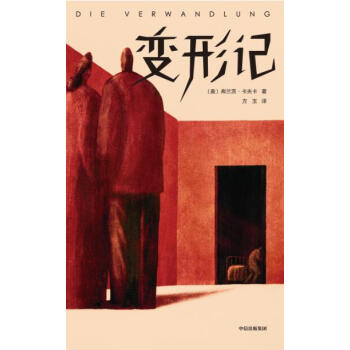
\includegraphics[width = .5\textwidth]{./ch/34.jpg}

\end{figure}



我睁开双眼发现四周漆黑一片,我努力的蠕动身体,终于一缕阳光照进了我的眼帘。我拼命地探出小脑袋,好想跟面前的世界亲近。我扒开土壤,把脑袋抬得很高,看向远方,希望看得更远一些。



阳光暖暖的照在我脸上,我美滋滋都享受着。中午我被太阳欺负时,旁边的树哥哥总会出来帮我阻挡,他的影子照在我身上,使我格外舒服。风儿姐姐也会出来帮我,她“呼、呼……”地吹,用她的方式来帮助我,好像要把太阳给吹跑似的。



我慢慢长大,身上长出了许多雪白的小花,我厌倦了这种无味的生活。



我对风儿姐姐说:“风儿姐姐,我想去远处看看,可能送我一程吗?”我知道风儿姐姐也舍不得我,但孩子最终也要长大。风儿姐姐选择了放手,大树哥哥也没有阻挡,而是随我漂流。风儿姐姐深深地吸了一口气,费了的九牛二虎之力,才吹了出去,我飞了起来,飞向了远方,那是我的理想,我要飞向更远地方。



我飞到高山上,大声呼喊地上的小草。小草听见了,也随之摇动起来,向我招手示好,我也对着小草招了招手;我飞到了一条小河上,小河拼命地奔跑,我对小河笑了笑,小河也对我笑了笑,我便不再打扰小河,静静地离开了;我飞到一处长满野草的小池塘,这时小动物们正在开派对呢!蝉井井有条的吹着口哨,在给声音铿锵有力的青蛙伴着激情的节奏,蝈蝈正在旁边弹着钢琴,连围观的野草也在旁边舞动着身体,热情的他们邀请路过的伙伴来参加,我拒绝了,因为我还要看更远的世界。



直到一天我累了,我尽最后一点力气停在了一个小区的花坛里,那里有许许多多的花。我沉沉地睡去,没有在睁开过双眼。不久之后,花坛里冒出一株蒲公英。



人生就是如此,只有不停的追求目标,不断的去实现,才会更加的多姿多彩。





\vspace{10pt}



作者:六(3) 孙媛媛



指导老师:刘嘉蕾



投稿:2021年4月27日



发表:2021年4月28日








                



\vspace{10pt}

\hline



